\documentclass[dvipsnames, tikz]{standalone}
\usepackage{amsmath}
\usepackage{arevmath}
\usepackage{xcolor}
\usepackage{tikz}
\usetikzlibrary{calc}
\usetikzlibrary{decorations.pathreplacing,calligraphy,3d}
\usetikzlibrary{matrix,shapes,fit,backgrounds}

\begin{document}
	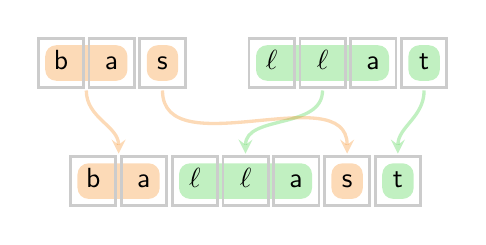
\begin{tikzpicture}[
		%Global config
		>=latex,
		line width=1pt,
		color = black,
		every left delimiter/.style={xshift=1ex},
		every right delimiter/.style={xshift=-1ex},
		%Styles
		Vector/.style={
			matrix of nodes,
			text height=1.85ex,
			text depth=0.75ex,
			text width=2.25ex,
			align=center,
			%left delimiter=(,
			%right delimiter=),
			column sep=1pt,
			row sep=1pt,
			nodes={draw=black!20}, % Uncoment to see the square nodes.
			%nodes in empty cells,
		},
		Matrix/.style={
			matrix of nodes,
			%text height=2.5ex,
			%text depth=0.75ex,
			%text width=3.25ex,
			%align=center,
			left delimiter=(,
			right delimiter=),
			%column sep=1pt,
			%row sep=1pt,
			%nodes={draw=black!10}, % Uncoment to see the square nodes.
			%nodes in empty cells,
		},
		DA/.style={
			fill,
			opacity=0.3,
			rounded corners,
			inner sep=-3pt,
			line width=1pt,
		},
		DG/.style={
			%line cap = round,
			%rounded corners=0.25ex,
			line width = 16pt,
			opacity = 0.3,
		}
		]
		
		\matrix[Vector] at (0,0) (M){ % Matrix contents  
			\sf b & \sf a & \sf s\\
		};
		
		\matrix[Vector] at (3,0) (N){ % Matrix contents  
			\sf $\ell$ & \sf $\ell$ & \sf a & \sf t\\
		};
	
		\matrix[Vector] at (1.7,-1.5) (O){ % Matrix contents  
			\sf b & \sf a & \sf $\ell$ & \sf $\ell$ & \sf a & \sf s & \sf t\\
		};
	
		\begin{scope}[on background layer] 
			%To delimit internal area groups
			%\node[DA,blue,fit=(M-3-2)(M-5-4)](subM-2){};
			\node[DA,BurntOrange,fit=(M-1-1)(M-1-2)](subM-1){};
			\node[DA,BurntOrange,fit=(O-1-1)(O-1-2)](subO-1){};
			
			\node[DA,LimeGreen,fit=(N-1-1)(N-1-3)](subN-1){};
			\node[DA,LimeGreen,fit=(O-1-3)(O-1-5)](subO-2){};
			
			\node[DA,BurntOrange,fit=(M-1-3)(M-1-3)](subM-2){};
			\node[DA,BurntOrange,fit=(O-1-6)(O-1-6)](subO-3){};
			
			\node[DA,LimeGreen,fit=(N-1-4)(N-1-4)](subN-2){};
			\node[DA,LimeGreen,fit=(O-1-7)(O-1-7)](subO-4){};
			
			% For line sectors		
			\draw[BurntOrange, very thick, -stealth, opacity=0.3] ([yshift=-3pt]subM-1.south) to[out=-90, in=90] ([yshift=3pt]subO-1.north);   
			\draw[LimeGreen, very thick, -stealth, opacity=0.3] ([yshift=-3pt]subN-1.south) to[out=-90, in=90]  ([yshift=3pt]subO-2.north);   
			\draw[BurntOrange, very thick, -stealth, opacity=0.3] ([yshift=-3pt]subM-2.south) to[out=-90, in=90]  ([yshift=3pt]subO-3.north);   
			\draw[LimeGreen, very thick, -stealth, opacity=0.3] ([yshift=-3pt]subN-2.south) to[out=-90, in=90]  ([yshift=3pt]subO-4.north);   
			%\draw[DG,NavyBlue](M-1-2.center) --(M-3-4.center);
			%\draw[DG,PineGreen](M-1-3.center) --(M-2-4.center);
			%\draw[DG,BrickRed](M-2-1.center) --(M-3-2.center);
			%\draw[DG,BurntOrange](M-3-1.center) --(M-3-1.center);
			%\draw[DG,LimeGreen](M-1-4.center) --(M-1-4.center);
		\end{scope}
		
	\end{tikzpicture}
\end{document}